\subsection{7 Sites Results}

The 3 sites cases, although is based on reality, already contains
some pooling effect initially due to some site has more than one
machines. We'd like to isolate out the impact of just diversions. Thus
it makes sense to conduct experiment on the case where instead of
having some big sites and small sites, we have 7 small sites, each
with one machine. This system has worse performance to begin with
because no pooling effect is present initially. Let's look at the
impact of diversions. Note all sites are totally homogeneous now:
they have same number of machines, same amount of load and
same open time. As a result, we don't need to look at system
performance at per site level.

\begin{figure}[htp]
\centering
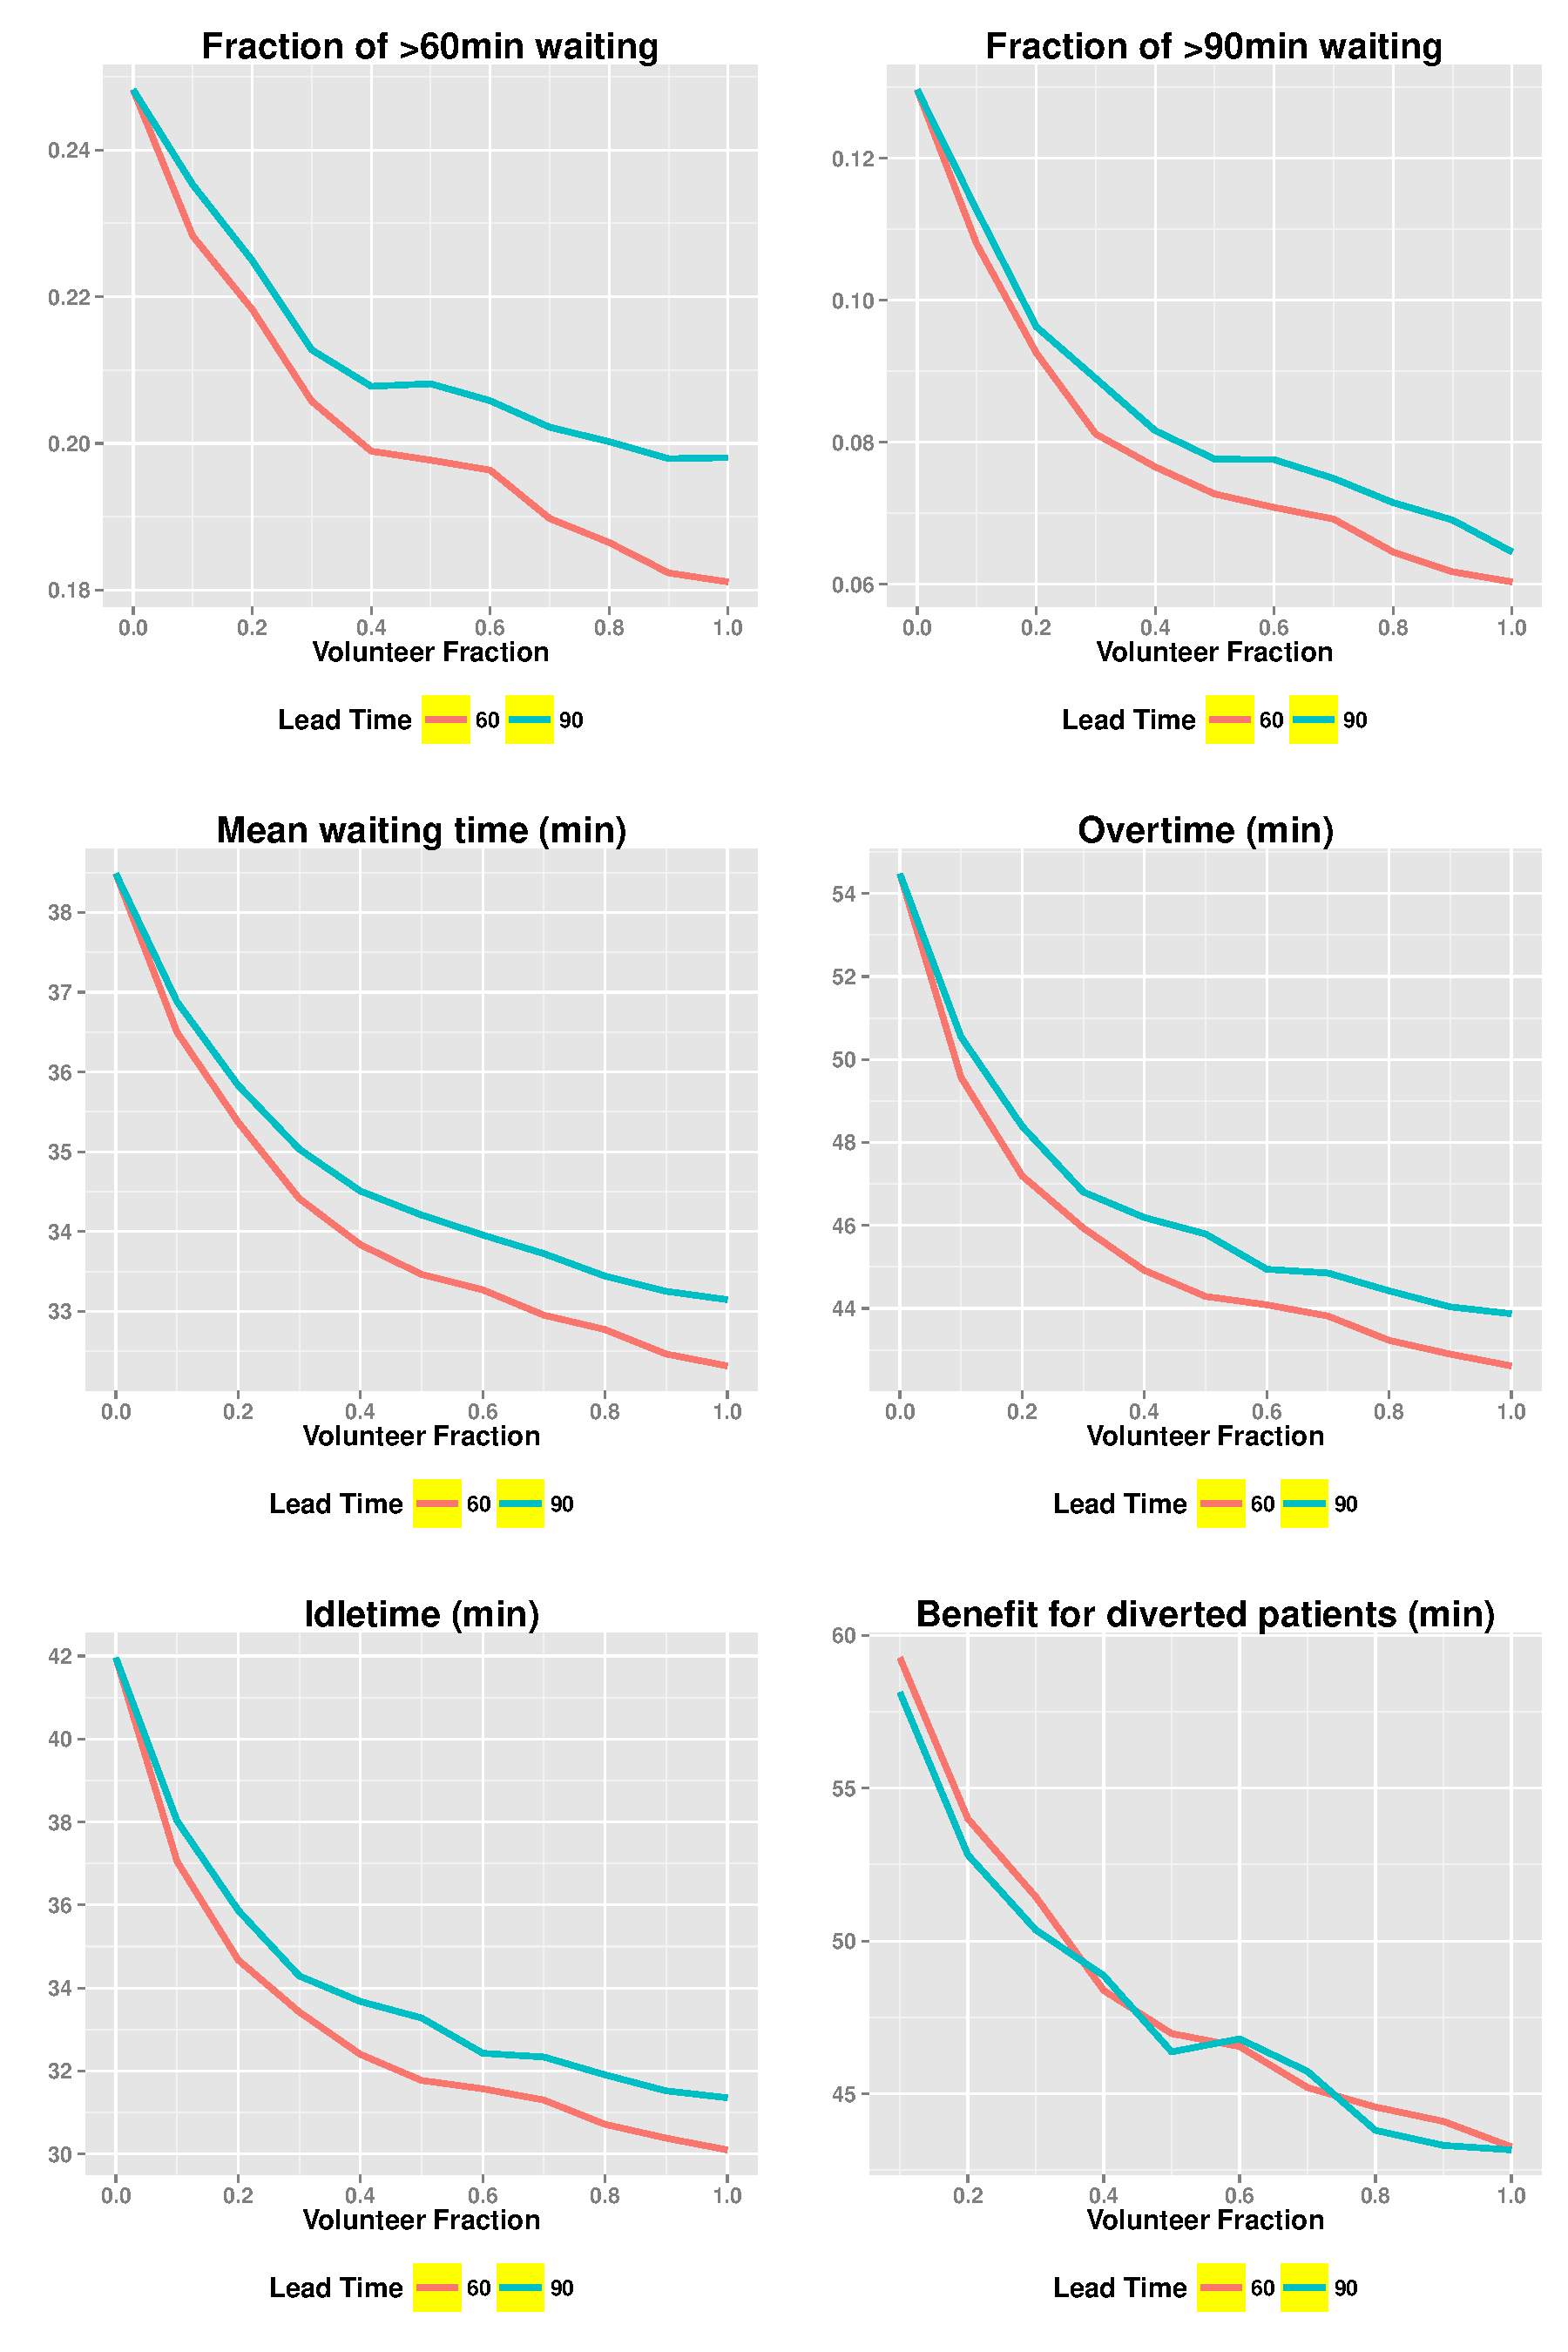
\includegraphics[width=.96\textwidth]{chap3/numeric/pic/7sites_all}
\caption{The impact of diversions on system performance of a system
with 7 sites, each with one machine.}
\label{fig:7sites_all}
\end{figure}

Figure \ref{fig:7sites_all} shows that compared to 3 sites case,
diversions have more impact on this system. This time, we have
significant improvement even on mean waiting time. This is exactly
because diversions bring pooling effect which is intially not
presented.

\begin{figure}[htp]
\centering
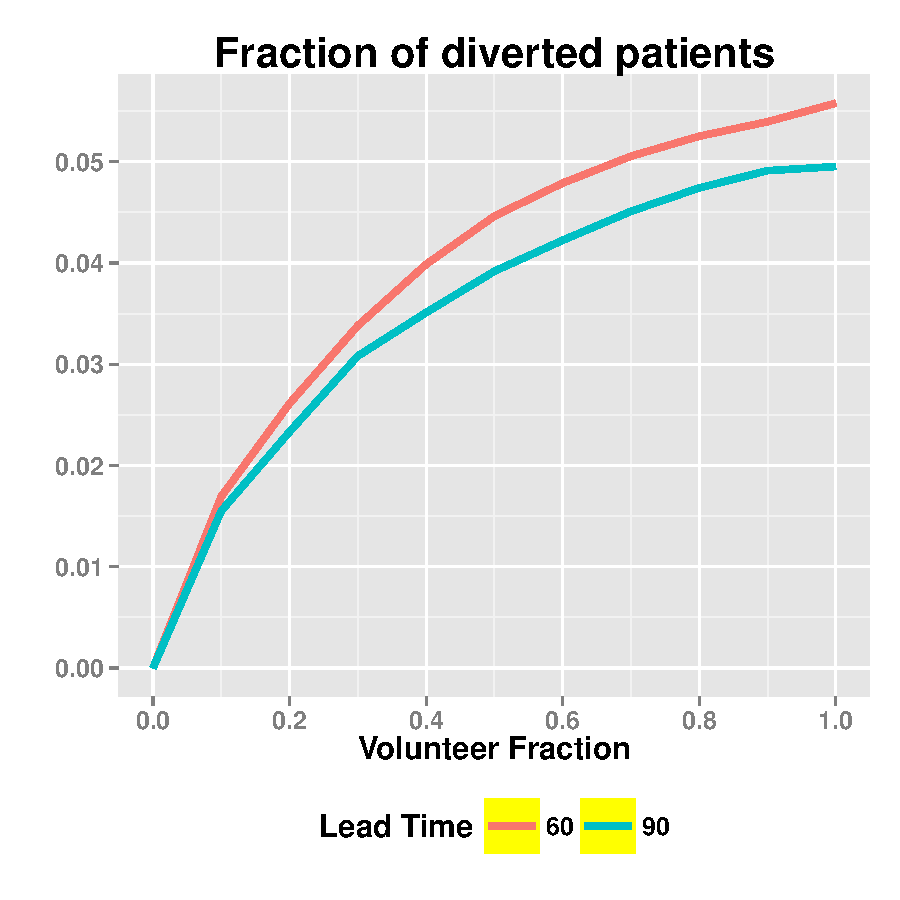
\includegraphics[width=.6\textwidth]{chap3/numeric/pic/7sites_all_diversion}
\caption{Fraction of diverted patients in 7 sites case.}
\label{fig:7sites_all_diversion}
\end{figure}

From Figure \ref{fig:7sites_all_diversion}, we see that we may potentially
divert 6\% patients if everyone is volunteer. This is a lot more compared
with 3 sites case. This shows that there are a lot more
beneficial diversion opportunities when there is no pooling initially. Also, for
diverted patients, each of them also enjoys more waiting time reduction
compared to 3 sites case.

Overall, the experiments for the 7 site confirms that greater benefit can
be achieved in the system with many small sites.
